\ifdefined\included
\else
\documentclass[a4paper,11pt,twoside]{StyleThese}
\usepackage{amsmath,amssymb}             % AMS Math
\usepackage[french]{babel}
\usepackage[utf8]{inputenc}
\usepackage[T1]{fontenc}
\usepackage{tabularx}
%\usepackage{tabular}
\usepackage{multirow}


\usepackage[tight,footnotesize]{subfigure}
\usepackage{algorithm} %To allow algorithm environment
\usepackage{algpseudocode} %Provides algorithmic environment

\usepackage{hhline}
\usepackage[left=1.5in,right=1.3in,top=1.1in,bottom=1.1in,includefoot,includehead,headheight=13.6pt]{geometry}
\renewcommand{\baselinestretch}{1.05}

% Table of contents for each chapter

\usepackage[nottoc, notlof, notlot]{tocbibind}
\usepackage[french]{minitoc}
\setcounter{minitocdepth}{2}
\mtcindent=15pt
% Use \minitoc where to put a table of contents

\usepackage{aecompl}

% Glossary / list of abbreviations

\usepackage[intoc]{nomencl}
\renewcommand{\nomname}{Liste des Abréviations}

\makenomenclature

% My pdf code

\usepackage{ifpdf}

\ifpdf
  \usepackage[pdftex]{graphicx}
  \DeclareGraphicsExtensions{.jpg}
  \usepackage[a4paper,pagebackref,hyperindex=true]{hyperref}
  \usepackage{tikz}
  \usetikzlibrary{arrows,shapes,calc}
\else
  \usepackage{graphicx}
  \DeclareGraphicsExtensions{.ps,.eps}
  \usepackage[a4paper,dvipdfm,pagebackref,hyperindex=true]{hyperref}
\fi

\graphicspath{{.}{images/}}

%nicer backref links
\renewcommand*{\backref}[1]{}
\renewcommand*{\backrefalt}[4]{%
\ifcase #1 %
(Non cité.)%
\or
(Cité en page~#2.)%
\else
(Cité en pages~#2.)%
\fi}
\renewcommand*{\backrefsep}{, }
\renewcommand*{\backreftwosep}{ et~}
\renewcommand*{\backreflastsep}{ et~}

% Links in pdf
\usepackage{color}
\definecolor{linkcol}{rgb}{0,0,0.4} 
\definecolor{citecol}{rgb}{0.5,0,0} 
\definecolor{linkcol}{rgb}{0,0,0} 
\definecolor{citecol}{rgb}{0,0,0}
% Change this to change the informations included in the pdf file

\hypersetup
{
bookmarksopen=true,
pdftitle="Évaluation de la sécurité des équipements grand public connectés à Internet",
pdfauthor="Yann BACHY", %auteur du document
pdfsubject="Thèse", %sujet du document
%pdftoolbar=false, %barre d'outils non visible
pdfmenubar=true, %barre de menu visible
pdfhighlight=/O, %effet d'un clic sur un lien hypertexte
colorlinks=true, %couleurs sur les liens hypertextes
pdfpagemode=None, %aucun mode de page
pdfpagelayout=SinglePage, %ouverture en simple page
pdffitwindow=true, %pages ouvertes entierement dans toute la fenetre
linkcolor=linkcol, %couleur des liens hypertextes internes
citecolor=citecol, %couleur des liens pour les citations
urlcolor=linkcol %couleur des liens pour les url
}

% definitions.
% -------------------

\setcounter{secnumdepth}{3}
\setcounter{tocdepth}{2}

% Some useful commands and shortcut for maths:  partial derivative and stuff

\newcommand{\pd}[2]{\frac{\partial #1}{\partial #2}}
\def\abs{\operatorname{abs}}
\def\argmax{\operatornamewithlimits{arg\,max}}
\def\argmin{\operatornamewithlimits{arg\,min}}
\def\diag{\operatorname{Diag}}
\newcommand{\eqRef}[1]{(\ref{#1})}

\usepackage{rotating}                    % Sideways of figures & tables
%\usepackage{bibunits}
%\usepackage[sectionbib]{chapterbib}          % Cross-reference package (Natural BiB)
%\usepackage{natbib}                  % Put References at the end of each chapter
                                         % Do not put 'sectionbib' option here.
                                         % Sectionbib option in 'natbib' will do.
\usepackage{fancyhdr}                    % Fancy Header and Footer

% \usepackage{txfonts}                     % Public Times New Roman text & math font
  
%%% Fancy Header %%%%%%%%%%%%%%%%%%%%%%%%%%%%%%%%%%%%%%%%%%%%%%%%%%%%%%%%%%%%%%%%%%
% Fancy Header Style Options

\pagestyle{fancy}                       % Sets fancy header and footer
\fancyfoot{}                            % Delete current footer settings

%\renewcommand{\chaptermark}[1]{         % Lower Case Chapter marker style
%  \markboth{\chaptername\ \thechapter.\ #1}}{}} %

%\renewcommand{\sectionmark}[1]{         % Lower case Section marker style
%  \markright{\thesection.\ #1}}         %

\fancyhead[LE,RO]{\bfseries\thepage}    % Page number (boldface) in left on even
% pages and right on odd pages
\fancyhead[RE]{\bfseries\nouppercase{\leftmark}}      % Chapter in the right on even pages
\fancyhead[LO]{\bfseries\nouppercase{\rightmark}}     % Section in the left on odd pages

\let\headruleORIG\headrule
\renewcommand{\headrule}{\color{black} \headruleORIG}
\renewcommand{\headrulewidth}{1.0pt}
\usepackage{colortbl}
\arrayrulecolor{black}

\fancypagestyle{plain}{
  \fancyhead{}
  \fancyfoot{}
  \renewcommand{\headrulewidth}{0pt}
}

%\usepackage{MyAlgorithm}
%\usepackage[noend]{MyAlgorithmic}
\usepackage[ED=MITT - STICIA, Ets=INP]{tlsflyleaf}
%%% Clear Header %%%%%%%%%%%%%%%%%%%%%%%%%%%%%%%%%%%%%%%%%%%%%%%%%%%%%%%%%%%%%%%%%%
% Clear Header Style on the Last Empty Odd pages
\makeatletter

\def\cleardoublepage{\clearpage\if@twoside \ifodd\c@page\else%
  \hbox{}%
  \thispagestyle{empty}%              % Empty header styles
  \newpage%
  \if@twocolumn\hbox{}\newpage\fi\fi\fi}

\makeatother
 
%%%%%%%%%%%%%%%%%%%%%%%%%%%%%%%%%%%%%%%%%%%%%%%%%%%%%%%%%%%%%%%%%%%%%%%%%%%%%%% 
% Prints your review date and 'Draft Version' (From Josullvn, CS, CMU)
\newcommand{\reviewtimetoday}[2]{\special{!userdict begin
    /bop-hook{gsave 20 710 translate 45 rotate 0.8 setgray
      /Times-Roman findfont 12 scalefont setfont 0 0   moveto (#1) show
      0 -12 moveto (#2) show grestore}def end}}
% You can turn on or off this option.
% \reviewtimetoday{\today}{Draft Version}
%%%%%%%%%%%%%%%%%%%%%%%%%%%%%%%%%%%%%%%%%%%%%%%%%%%%%%%%%%%%%%%%%%%%%%%%%%%%%%% 

\newenvironment{maxime}[1]
{
\vspace*{0cm}
\hfill
\begin{minipage}{0.5\textwidth}%
%\rule[0.5ex]{\textwidth}{0.1mm}\\%
\hrulefill $\:$ {\bf #1}\\
%\vspace*{-0.25cm}
\it 
}%
{%

\hrulefill
\vspace*{0.5cm}%
\end{minipage}
}

\let\minitocORIG\minitoc
\renewcommand{\minitoc}{\minitocORIG \vspace{1.5em}}

\usepackage{multirow}
%\usepackage{slashbox}

\newenvironment{bulletList}%
{ \begin{list}%
	{$\bullet$}%
	{\setlength{\labelwidth}{25pt}%
	 \setlength{\leftmargin}{30pt}%
	 \setlength{\itemsep}{\parsep}}}%
{ \end{list} }

\newtheorem{definition}{Définition}
\renewcommand{\epsilon}{\varepsilon}

% centered page environment

\newenvironment{vcenterpage}
{\newpage\vspace*{\fill}\thispagestyle{empty}\renewcommand{\headrulewidth}{0pt}}
{\vspace*{\fill}}

\usepackage{tablefootnote}
\sloppy
\begin{document}
\setcounter{chapter}{3} %% Numéro du chapitre précédent ;)
\dominitoc
\faketableofcontents
\fi

\chapter{Prise de Perspective et Reconnaissance d'Intentions}
\label{chapter4}
\minitoc

\section{Contexte}
%ROMAN 2016
Créer des systèmes capables d'interagir avec l'humain de façon efficace et qui paraisse naturelle et intuitive à l'homme est une des problématiques essentielles de la robotique d'assistance. Dans leurs activités quotidiennes, les humains collaborent régulièrement sans avoir besoin de requête explicites ou de communication verbale. Une compétence importante pour accomplir cela est la capacité de déduire les croyances et les intentions des autres à partir d'observations et d'indices contextuels. Afin d'être efficace, socialement cohérent et d'aider au mieux l'homme, la connaissance des croyances et la reconnaissance d'intention sont des fonctionnalités importantes à fournir aux robots qui coopèrent ou assistent les humains.

Pour illustrer le problème, nous prenons un scénario. Imaginons une femme, appelée Alice. Alice a finit sa journée de travail et rentre à sa maison. Alice aimerait se détendre en lisant un peu. Elle se mets sur le sofa avec un livre et se dirige vers une table à proximité pour prendre ses lunettes. Elle ignore que son mari, pendant la journée, a déplacé ses lunettes dans une autre pièce.
Imaginons à présent un robot domestique dans cette situation, qui passe sa journée dans la maison, se déplaçant entre les pièces et essayant d'aider la famille le plus possible. Pour aider les humains, ce robot devrait être doté de plusieurs capacités motrices, perceptuelles, et cognitives. Le robot devrait bien évidemment pouvoir percevoir la présence des humains et des objets de l'environnement, se déplacer librement, et interagir avec les objets.

Pour être un assistant efficace, le robot devrait également être capable de comprendre les problèmes et objectifs des humains. Dans cette situation, il devrait être capable d'analysé qu'Alice, après une journée fatigante, désire se détendre en lisant un livre, qu'elle a besoin pour cela de ses lunettes, et qu'elle ignore la position de celles-ci car son mari les a déplacées. Si le robot avait ces compétences, il pourrait aller chercher les lunettes d'Alice et les lui apporter sans demande spécifiques de sa part, faisant de lui un assistant de vie discret, proactif et efficace.

%%INTENTIONS
Un des aspects clés dans le scénario présenté est la capacité du robot à savoir qu'Alice ignore que ses lunettes ne sont plus où elle les a laissées. Sans cette connaissance, le robot aurait probablement estimé qu'Alice cherchait à prendre un objet présent sur la table. 
Il semble que, pour interagir avec les humains, les robots ont besoin d'avoir un ensemble de capacités qui leur permettent de comprendre et modéliser les croyances des utilisateurs, afin d'interpréter leurs actions et d'ainsi permettre la reconnaissance de plan. Une approche pour résoudre ce problème est d'étudier les mécanismes utilisés par les humains lorsqu'ils interagissent entre eux, et essayer de les adapter dans des scénarios de robotique afin de rendre le processus d'interaction homme-robot le plus naturel et intuitif possible pour les humains.

Le premier point qu'il nous faut introduire est le concept d'intention. Il y a beaucoup de définitions différentes de l'intention dans la littérature psychologique  \cite{bruner1981} et philosophique \cite{bratman1984}. Ici, nous définissons une intention comme étant le souhait et la volonté d'atteindre un objectif. L'intention émerge de causes contextuelles (motivations) et reste présente jusqu'à ce que l'objectif soit atteint ou abandonné, poussant l'agent à entreprendre des actions menant à cet objectif.

Comprendre correctement les intentions d'autrui requiert de raisonner sur leurs croyances et leurs pensées afin d'interpréter correctement leurs actions. Cette compétence est la théorie de l'esprit et la capacité de prise de perspective associée, présentée au chapitre \ref{chapter2}.

% %b in robotics
% Previous works in robotics have shown that enhancing the robot's perspective taking abilities improves its reasoning capabilities, leading to more appropriate and efficient task planning and interaction strategies \cite{breazeal2006,Trafton2005}.
% % Among others, ~\cite{breazeal2006} presents a learning algorithm that takes into account information about a teacher's visual perspective in order to learn specific colored buttons activation/deactivation patterns, and ~\cite{Trafton2005} uses both visual
% % and spatial perspective taking to find out the referent
% % indicated by a human partner.
% An important study linked to conceptual perspective taking is the 'divergent belief task'.  Formulated in~\cite{wimmer1983}, this kind of task requires the ability to recognize that others can have beliefs about the world that differ from the observable reality.
Ainsi, Breazeal dans \cite{BreazealGB09}, propose d'utiliser cette prise de perspective pour la reconnaissance de but. Cette capacité de prise de perspective est une prérogative pour la reconnaissance d'intention, car, comme expliqué par \cite{byom2013theory}, "en tant qu'humains nous croyons généralement que les autres agissent de façons cohérentes avec leurs croyances et leurs objectifs". Il est donc nécessaire que l'interprétation des actions de l'homme soit basée sur leur état de croyance pour déduire correctement leur intention. Ainsi dans \cite{Call1998} les sujets sont capables d'interpréter les actions d'autres humains pour distinguer une action "intentionnelle" d'une action "accidentelle".

La reconnaissance des activités humaines est un sujet important dans la recherche en sciences informatiques, et elle peut être étudiée à différents niveaux. L'anticipation des actions humaines et des mouvements permet au robot d'adapter son comportement et d'aider l'humain de façon proactive, comme étudié dans \cite{koppula2013anticipating}. Une idée intéressante est d'utiliser les modèles internes du robot lui-même pour reconnaître les actions et prédire l'intention de l'utilisateur, comme montré par le système \textit{HAMMER} dans \cite{demiris2007prediction}. 

Les séquences d'actions peuvent être liées à des plans. Ceci constitue une thématique de recherche appelée la reconnaissance de plan. Plusieurs approches ont été étudiées dans ce domaine, en utilisant par exemple la planification classique \cite{ramirez2009plan}, probabiliste \cite{bui2003general} ou des techniques logiques \cite{singla2011abductive}. Une infrastructure logicielle intéressante pour la reconnaissance d'intention est la théorie de l'esprit Bayésienne \cite{baker2014modeling}, utilisée pour représenter les processus de déduction d'un observateur regardant le comportement d'un autre agent, basée sur des POMDPs et des réseaux Bayésiens dynamiques (DBN for Dynamic Bayesian Networks).

Deux approches qui peuvent être utilisées pour l'estimation d'intention sont les processus interactifs de Markov partiellement observés (I-POMDP pour Interactive Partially Observed Markov Decision Processes) et l'apprentissage inverse. Les I-POMDP \cite{gmytrasiewicz2004interactive} offrent un cadre riche qui étend les processus de décision de Markov partiellement observés (POMDP) dans un cadre multi-agent. Les déductions dans ces modèles peuvent être extrêmement complexes, mais il y a eu des tentatives pour résoudre ce problème, comme dans \cite{doshi2009monte, hoang2013interactive}.


%The problem of plan inference in large  models with many features was addressed in \cite{Krauthausen2010}, using the technique of model switching on Dynamic Bayesian Networks (DBN).

%Interactive Partially Observed Markov Decision Processes \cite{gmytrasiewicz2004interactive} offer a rich framework that extends Partially Observed Markov Decision Processes (POMDP) in a multi-agent setting. Inference in these models can be extremely complex, but there have been attempts at solving this issue, like in \cite{doshi2009monte,hoang2013interactive}. 
%The problem of plan inference in large  models with many features was addressed in \cite{Krauthausen2010}, using the technique of model switching on Dynamic Bayesian Networks (DBN).


L'apprentissage inverse par renforcement \cite{ng2000algorithms} formule le problème de calcul d'une fonction de récompense inconnue d'un agent après avoir observé son comportement. Cette stratégie a été appliquée, en utilisant des réseaux bayésiens (BN), dans \cite{Nagai2015} afin d'apprendre le modèle mental d'un autre agent, et choisir les actions appropriées pour une tâche visant à établir une relation. Une approche liée est la planification inverse, qui a été appliquée dans une infrastructure bayésienne dans \cite{baker2009action} pour la compréhension de l'action humaine.

Les informations contextuelles peuvent être également utilisées pour mieux résoudre des situations complexes. \cite{Liu2014} montre un système qui utilise des BNs pour comprendre les intentions des utilisateurs avec une importance tout particulière portée aux données contextuelles.

%%IV Robot reactions
Les robots assistants ont besoin non seulement de prédire les intentions humaines, mais aussi de produire des plans socialement acceptables afin de les aider à atteindre leur but. Certains systèmes, comme Pike \cite{karpas2015robust} et Chaski \cite{shah2011improved}, modélisent explicitement les humains dans leurs plans et permettent au robot d'adapter son comportement aux actions des utilisateurs. D'autres approches, telles que \cite{levine2014concurrent}, intègrent les actions du robot dans le processus de reconnaissance, ce qui permet au système d'adapter avec souplesse son plan pour les humains.

Bien qu'il existe plusieurs travaux intéressants liés au problème de la reconnaissance de l'intention, nous croyons que, pour le moment, peu de systèmes intègrent ces mécanismes dans une architecture complète, capable de représenter et de suivre les modèles mentaux des agents, de reconnaître les intentions, de gérer des plans collaboratifs et d'agir de façon proactive. Dans \cite{talamadupula2014coordination}, les auteurs utilisent la planification classique, avec une stratégie de replanification efficace, afin d'en déduire les intentions de l'utilisateur. Le système a été mis en œuvre sur un robot PR2 et testé sur un scénario de collaboration. \cite{breazeal2009embodied} présente une architecture dans laquelle le robot est capable d'utiliser ses propres schémas et modèles pour déduire les actions et les objectifs humains et d'aider activement à les atteindre. Les plans partagés ne sont pas explicitement représentés dans le système, et le robot aide l'humain en faisant correspondre les informations de but inférées avec ses propres croyances, et en choisissant les actions appropriées.

L'une des contributions principale de ces travaux est l'introduction d'un module de reconnaissance d'intention basé sur le modèle de croyances des agents maintenu par notre système d'estimation de la situation. Ceci permet au robot d'interpréter correctement les intentions et d'aider de manière proactive et plus pertinente les humains (après avoir observé leurs comportements et en reconnaissant leurs intentions).
Notre algorithme de reconnaissance de l'intention est basé sur une intégration de BNs et MDPs, qui sont utilisés pour évaluer comment les actions humaines se rapportent à différents objectifs possibles tout en considérant leurs croyances. Nous introduisons le contexte comme information a priori, que nous avons appris de l'homme dans une approche similaire à \cite{Liu2014}. En utilisant le contexte, nous pourrions représenter, par exemple, que l'homme est plus susceptible de prendre un parapluie au cours d'une journée pluvieuse lorsqu'il sort de chez lui. Nous évaluons ce module dans une étude utilisateur, en comparant les compétences de reconnaissance de l'intention du robot avec celles des humains. Une autre de nos contributions est l'intégration de ce module dans une architecture robotique complète, permettant au robot d'aider de manière proactive les humains après l'estimation de leurs intentions les plus probables.

Notre système est basé sur plusieurs travaux antérieurs. Dans \cite{fioreiser2014}, nous avons présenté un système capable d'exécuter des actions conjointes avec les partenaires humains de manière flexible en adaptant le processus aux préférences de l'utilisateur. L'exécution de la modalité du système peut changer au cours d'un plan, ce qui permet au robot ou à l'humain d'assumer un rôle de leader ou de traiter les participants comme des partenaires égaux. Nous avons également montré dans les chapitres précédent comment nous étions capable de comprendre la situation de l'interaction et notamment de maintenir un modèle d'état mental distinct et cohérent pour chaque agent.

%Dans \cite{Milliez2014}, nous avons présenté un élément d'évaluation de la situation, capable de gérer des modèles distincts pour représenter les croyances états des agents et utilisé pour passer le test ~ \ Sally et Anne cite {Baron1985} sur une plate-forme robotique. Dans \ cite {Ferreira2015}, nous avons utilisé un composant de gestion de croyance avec un système de dialogue situé dans un simulateur. Ce modèle a été comparé à un système de base (sans prise de conscience de la croyance) dans une étude avec 60 interactions, dans un environnement simulé. Nous avons montré avec succès que le système de gestion du dialogue améliore considérablement son efficacité, ce qui réduit le nombre de tours du dialogue dans l'interaction, et sa précision, avec un taux de réussite plus élevé quand une situation de croyance divergente apparaît.

% Robot assistants need not only to predict human intentions, but also to produce socially acceptable plans in order to help them. Some systems, like Pike \cite{karpas2015robust} and Chaski \cite{shah2011improved}, explicitly model humans in their plans and allow the robot to adapt its behavior to the users' actions.  Other approaches, such as \cite{levine2014concurrent}, integrate robot's actions in the recognition process, allowing the system to flexibly adapt its plan to humans. 

% While there are several interesting works related to the intention recognition problem, we believe that, at the moment, few systems integrate these mechanism in a complete architecture, able to represent and track agent mental models, recognize intentions, produce collaborative plans, and act. In \cite{talamadupula2014coordination}, the authors use classical planning, with an efficient replanning strategy, in order to infer user's intentions. The system has been implemented on a PR2 robot and tested on a collaborative scenario. \cite{breazeal2009embodied} presents an architecture in which the robot is able to use its own schemas and models to infer human actions and goals, and to proactively help him achieve them. Shared plans are not explicitly represented in the system, and the robot helps the human by mapping the inferred goal information in its own beliefs, and choosing appropriate actions.

% The main contribution of this paper is introducing an intention recognition module, allowing the robot to proactively help humans, after observing their behaviors and recognizing their intentions.
% Our intention recognition algorithm is based on an integration of BNs and MDPs, which are used to evaluate how human actions relate to different possible goals. We introduce context as a-priori information, which we learnt from humans in a similar approach to \cite{Liu2014}. Using context we could represent, for example, that a human is more likely to take an umbrella during a rainy day. We evaluate this module in a user study, comparing the intention recognition skills of the robot with those of humans. Another of our contributions is integrating this module in a complete robotic architecture, enabling the robot to proactively help humans after estimating their most likely intentions.

% Our system is based on several  previous works. In \cite{fioreiser2014}, we presented a system able to execute joint actions with human partners in a flexible way by adapting the process to the user's preferences. The system's execution modality could change during a plan, allowing either the robot or the human to assume a leader role or treating participants as equal partners. In \cite{Milliez2014}, we presented a component for situation assessment, able to manage separate models to represent agents' belief states and used to pass the Sally and Anne test~\cite{Baron1985} on a robotic platform. In \cite{Ferreira2015}, we used a belief management component together with a situated dialogue system in a simulator. This model was compared with a basic system (without belief awareness) in a study with 60 interactions, in a simulated environment. We successfully showed that the dialogue management system significantly improves its efficiency, reducing the number of dialogue turns in the interaction, and its accuracy, with a higher success rate when a divergent belief situation appears.


\section{Estimation de l'intention}
\label{sec:intention_recognition}
Afin de déduire les intentions humaines, nous allons fournir les informations suivantes au système de reconnaissance: une liste de contextes connus, une liste des intentions connues, une liste d'actions connues, un ensemble d'observations de l'action humaine, et un modèle de croyance de l'homme et du robot.

Nous proposons, comme modèle central utilisé pour l'estimation de l'intention, une infrastructure logicielle basée sur des BNs. Un BN est un graphe orienté acyclique avec des variables aléatoires en tant que nœuds. Les connexions entre les nœuds représentent les dépendances conditionnelles entre les variables associées. Ainsi, on peut associer une fonction de probabilité à chaque nœud, dépendant de ses variables mères, qui produit la distribution de probabilité de la variable correspondante. Lorsque nous acquérons des informations, nous pouvons considérer une partie des nœuds comme \textit{preuves}, en fixant leur valeur, ce qui permet de produire une meilleure estimation des probabilités des autres nœuds. Nous appelons notre implémentation de BN un Graphe d'Intention (IG pour Intention Graph).

%In order to infer human intentions, we will provide the following information to the robot: a list of known contexts, a list of known intentions, a list of known actions, a set of observations of human action, and a belief model of humans and of itself.

%We propose, as central model used for intention estimation, a framework based on BNs. A BN is a directed acyclic graph with random variables as nodes. Edges between the nodes represent conditional dependencies between the associated variables. We can associate a probability function to each node, depending on its parent variables, that produces the probability distribution of the associated variable. When we acquire information we can consider a part of the nodes as \textit{evidence}, fixing their value and producing a better estimation of the other nodes' probabilities. We call our implementation of BN an Intention Graph (IG).
%Bayesian Networks support both "top-down" reasoning (i.e. casual, from causes to effects) and "bottom up" reasoning (i.e. diagnostic, from effects to causes). 
Un IG est composé des couches de nœuds suivants:
\begin{itemize}
\item Nœuds de Contexte: ces nœuds représentent les données contextuelles, modélisées par des booléens (e.g. HotDay, ColdDay).
\item Nœuds d'Intention: ces nœuds booléens représentent l'ensemble des intentions possibles. Chaque intention peut avoir une dépendance conditionnelle à plusieurs contextes.
%these boolean nodes represent the set of possible intentions. Each intention can conditionally depend on several contexts.
\item Nœuds d'Action. c'est l'ensemble des actions humaines qui sont actuellement surveillées. Chacun de ces nœuds a une dépendance conditionnelle à l'ensemble des nœuds d'intention.
\item Nœuds d'observation. Nous associons à chaque action un ensemble de nœuds d'observation particulier, qui ont une dépendance conditionnelle au nœud d'action en question. 
\end{itemize}


Dans une utilisation classique, le robot va créer, pour chaque humain "surveillé" (monitored human), un IG, formé par les nœuds de contexte et d'intention, que nous considérons statiquement connus par le robot, et une liste variable de nœuds d'action et d'observation, qui dépend du modèle de croyance de l'homme. Le système va créer un nœud d'action pour chaque action connue dont les  $preconditions$ sont satisfaites dans le modèle de croyance de l'humain, et leurs nœuds d'observation associées. L'IG de chaque agent devra être mis à jour chaque fois qu'un agent exécute une action A. Pour se faire, le système change dans chaque IG, les nœuds d'action et d'observation de la version précédent A pour les remplacer par de nouveaux, qui correspondent à l'état du monde après que A a été effectuée. En effet, chaque action modifiant l'État du monde, elle modifie potentiellement les actions possibles en validant ou invalidant certaines préconditions.

% In a typical usage, the robot will create, for each monitored human, an IG, formed by the Context and Intention Nodes, which we consider statically known by the robot, and a variable list of Action and Observation nodes, which depends on the human's belief model. The robot will create action nodes for each known action whose $preconditions$ are satisfied in the human's belief model, and their related Observation Nodes. These IGs will need to be updated every time that an agent performs an action, switching the previous Action and Observation nodes with new ones, that will depend on the state of the world after the action was performed.

Lors de la "surveillance" d'un humain par le système, nous utilisons les nœuds de contexte et d'observation comme \textit{preuves}, ce qui revient à les considérer comme observable par le robot. Ces informations nous permettent d'avoir une bonne estimation des actions et des intentions les plus probables pour l'homme, comme expliqué dans \ref{intention and action inference}.

Un exemple d'IG, pris d'une expérience, peut être vu dans la figure \ref{fig: intention_graph}. Dans les paragraphes qui suivent, nous allons expliquer le rôle de ces couches de nœuds, et comment les dépendances conditionnelles les reliant sont calculées.

% When monitoring a human, we set Context Nodes and Observation Nodes as \textit{evidence}, considering them observable by the robot. These information will allow us to have a good estimation of the most likely actions and intentions of the human, as explained in \ref{intentiom and action inference}.

% An example of IG, taken from an experiment, can be seen in figure \ref{fig:intention_graph}. In the following paragraphs, we will explain the role of these layers of nodes, and how the conditional dependencies between them are computed.

\vspace{-10pt}

 \begin{figure}[h!]
	\centering
	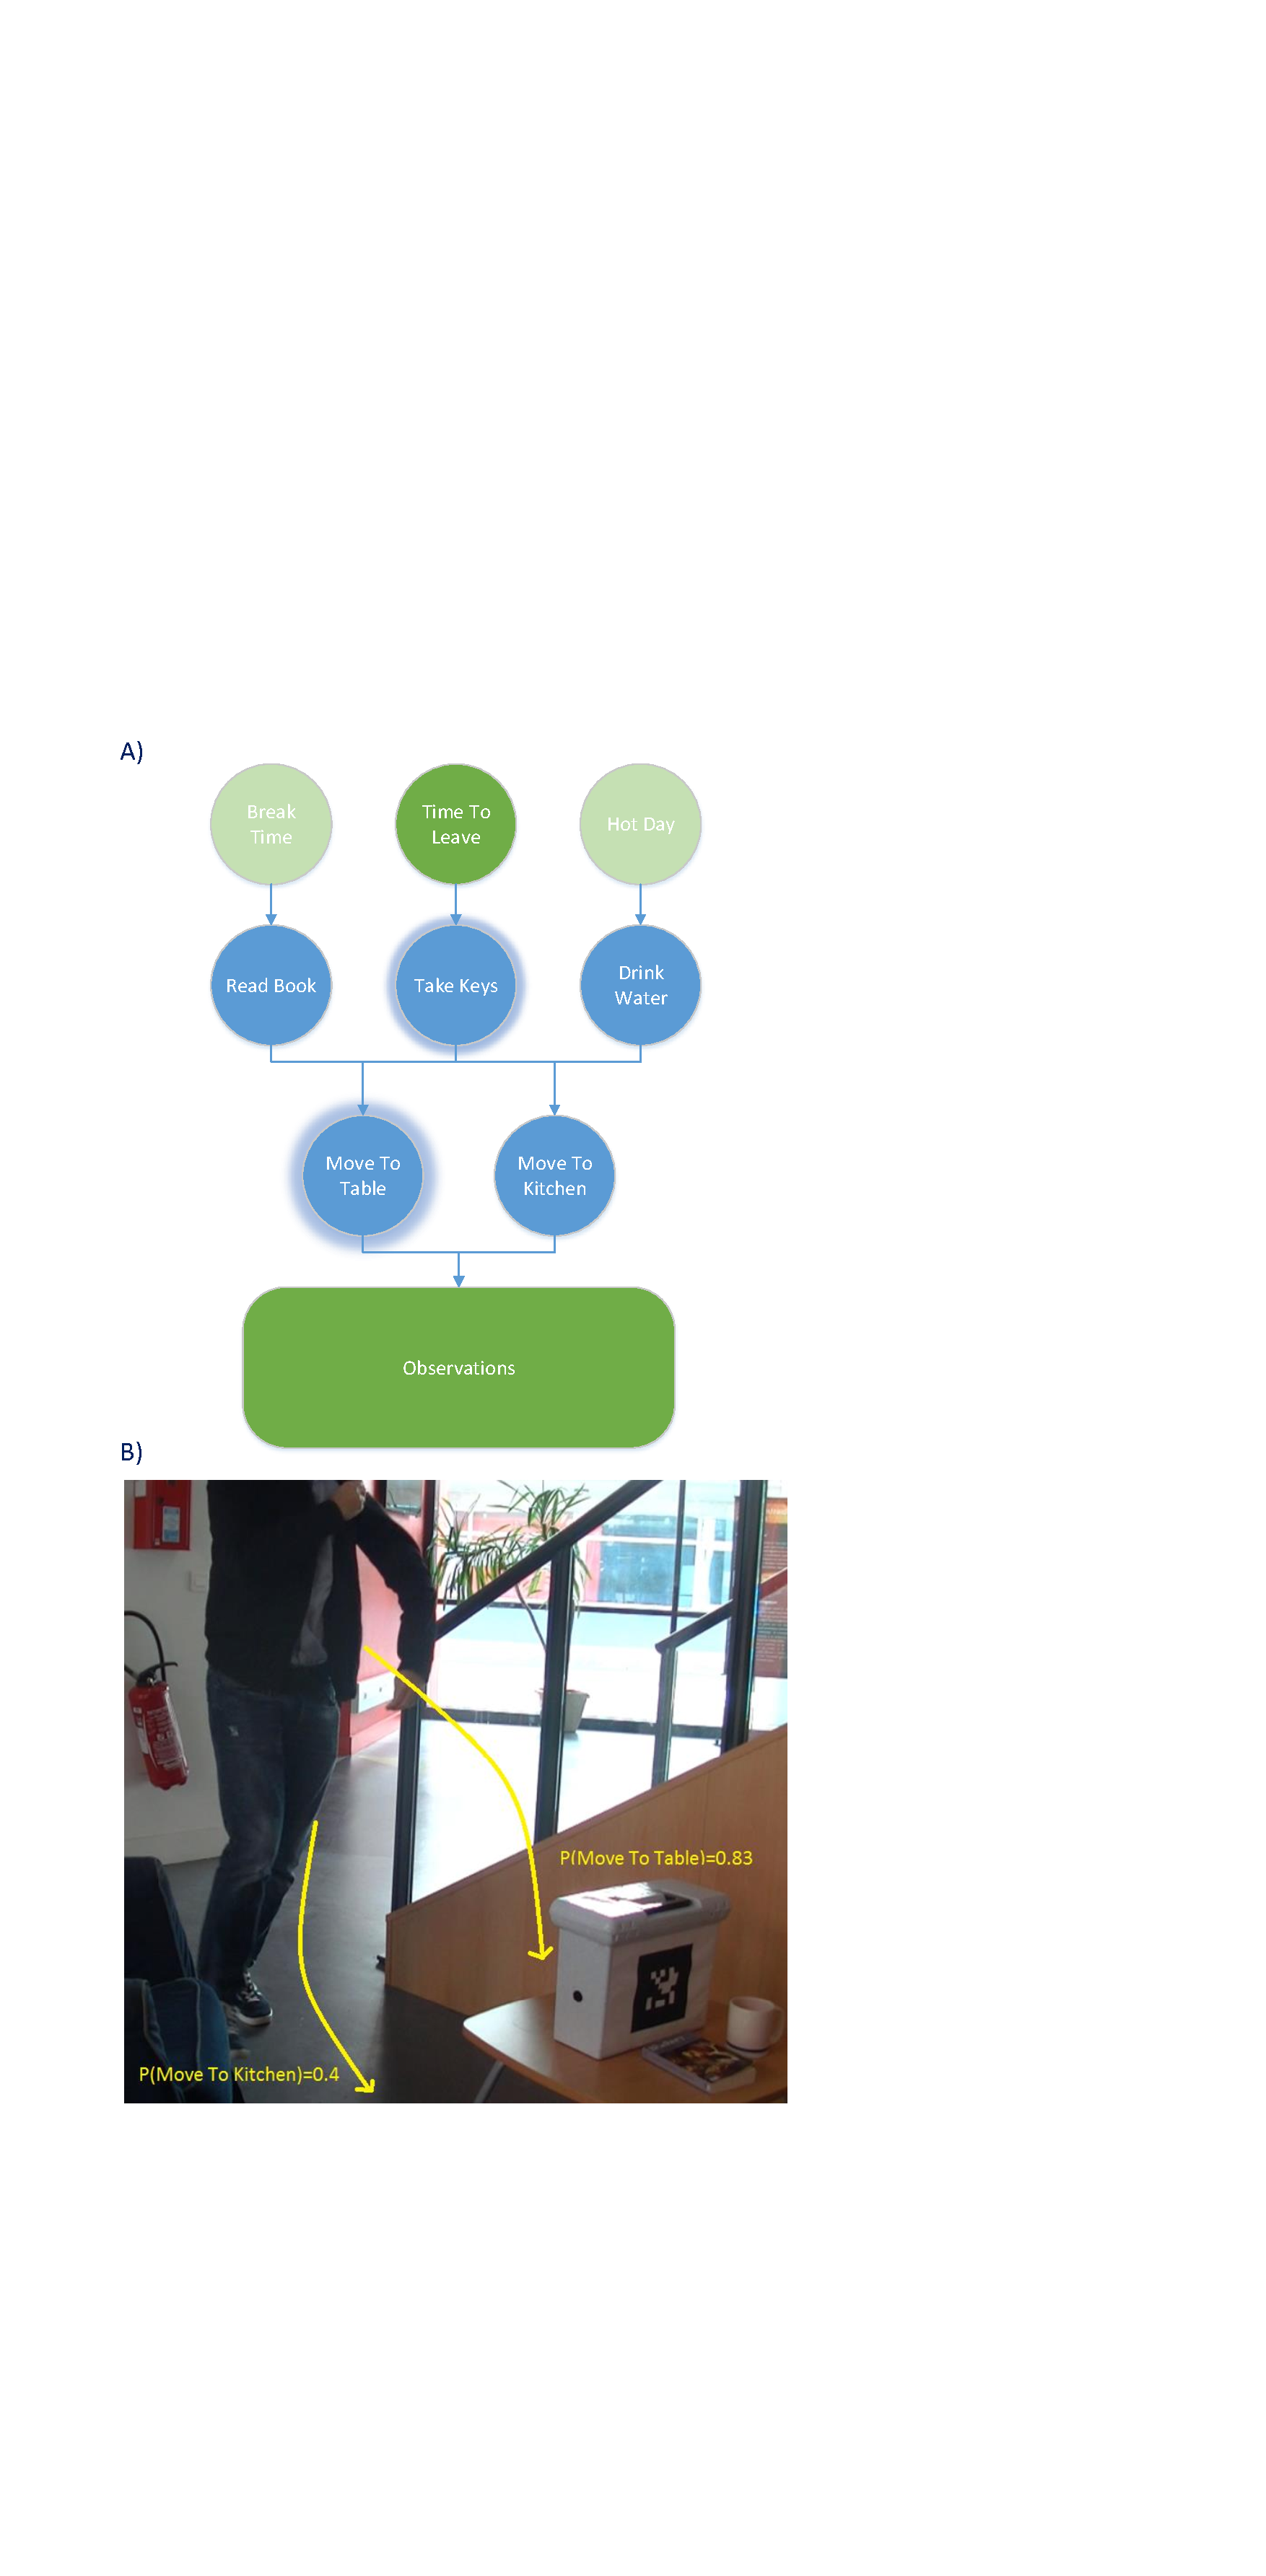
\includegraphics[trim={2cm 11cm 11cm 17cm},clip,scale=0.56]{img/cookieScenario.pdf}
	\caption{Une scène d'expérimentation. Les flèches jaunes montrent les actions possibles et leur probabilités associées. Le diagramme représente l'IG (Intention Graph) actuel. Les cercles verts représentent les nœuds considérés comme preuves et les bleus sont les autres nœuds. Pour les nœuds de contexte, situés en haut du graphe, les nœuds ayant une valeur fausse sont grisés. Pour les autres nœuds, ceux ayant la probabilité la plus forte sont entourés. Les nœuds d'observation ont étés regroupés en un seul bloque pour simplifier le diagramme.}
	\label{fig:intention_graph}
   	\vspace{-20pt}
\end{figure}

\subsection{Du contexte à l'intention}
Nous introduisons un ensemble de contextes dans notre domaine. Nous considérons comme contexte n'importe quelle information qui peut être utilisée pour caractériser et motiver une intention \cite{abowd1999towards}. Nous modélisons un contexte sous la forme d'une propriété, qui peut prendre différentes valeurs et influencer la probabilité d'un utilisateur d'avoir une intention donnée. Par exemple, on établit qu'un humain a plus de chance de vouloir cuisiner à l'heure du dîner, ou de boire une boisson chaude lorsqu'il fait froid.

Les nœuds de contexte peuvent directement influencer un ou plusieurs nœuds d'intention. Dans note approche, nous avons choisit d'apprendre ces dépendances conditionnelles directement de l'homme, comme expliqué dans la partie \ref{sec:expeRobotIntent}.

\subsection{De l'intention à l'action}
\label{action_evaluation}
Pour comprendre comment les actions sont liées aux intentions, il faut pouvoir répondre à la question: quelles actions ferait un humain, dans cette situation, étant donné son état de croyance sur l'état du monde, pour accomplir l'objectif lié à son intention? 
Notre démarche est basée sur le principe de rationalité \cite{Dennet1989}, qui affirme que les agents ont tendance à, étant donner leur état de croyance, choisir l'action qui leur semble la plus efficace, afin d'atteindre leur but.

Dans \cite{Blakemore2001}, les auteurs expliquent que "l'attribution des intentions aux actions pourrait reposer sur l'identification de l'action observée et sa correspondance dans notre propre représentation de l'intention". Nous suivons cette idée en donnant au robot un ensemble de modèles de planification. Chacun de ces modèles de planification est relié à une intention, et représente l'ensemble des plans associés permettant d'atteindre le but de l'intention. Grâce à cela, nous pouvons quantifier la correspondance de l'action humaine avec un plan donné, qui est lui même associé à une intention. En d'autres termes, cela permet de répondre à la question "Est-ce que l'humain pense que l'action qu'il vient de faire lui permet d'atteindre tel ou tel but lié à telle ou telle intention".

Dans notre implémentation, pour chaque intention connue par le système, nous créons un Processus de Décision Markovien (MDP pour Markov Decision Process) associé, pour représenter tous les plans possible liés à cette intention. Un MDP modélise le processus de décision pour un agent dans des situations où le résultat d'une action est partiellement aléatoire, et peut amener à plusieurs résultats. De façon formelle, un MDP est un tuple  \((Q,A,T,R,\gamma)\), où $Q$ est l'état du système, $A$ est un ensemble d'actions, $T(s,a,s')$ est la probabilité que réaliser l'action $a$ dans l'état $s$ mènera à un état $s'$, $R(s,a)$ est la récompense que l'agent obtiendra après avoir réalisé l'action $a$ dans l'état $s$ et \(\gamma\) est un facteur d'actualisation.

% In our implementation, for each intention known by the robot, we will create an associated Markov Decision Process (MDP), to represent all the possible plans associated to this intention. A MDP models the decision process of an agent in situations where the result of an action is partly random, and can lead to several outcomes. Formally a MDP is a tuple \((Q,A,T,R,\gamma)\), where $Q$ is the system state, $A$ is a set of actions, $T(s,a,s')$ is the probability that taking action $a$ in state $s$ will lead to state $s'$, $R(s,a)$ is the reward that the agent will gain after performing action $a$ in state $s$ and \(\gamma\) is a discount factor.

Le soucis principal des MDPs est de déterminer la fonction \(\pi(s)\) définissant la politique optimale qui associe la meilleur action à chaque état. "Meilleur" signifie ici que nous cherchons l'action qui maximise le gain de la récompense sur un horizon potentiellement infini. Il y a plusieurs algorithmes bien connus pour calculer la politique d'un MDP (voir \cite{2012Mausam}). En utilisant ces algorithmes nous pouvons également calculer, pendant l'apprentissage, la fonction de valeur d'action \(Q(s,a)\) qui associe à un état $s$ et une action $a$ la récompense attendue sur un horizon actualisé infini. Cette fonction est un point essentiel dans notre approche du problème d'estimation de l'intention.



Nous allons à présent expliquer comment nous utilisons la fonction de valeur d'action pour créer des dépendances conditionnelles entre nœuds d'intention et nœuds d'action dans l'IG. Commençons par définir \(P(a|I_i=1)\), la probabilité que l'action $a$ soit réalisée si l'intention $I_i$ est vraie. Nous modélisons cette probabilité comme \(P(a|I_i=1)=\frac{Q_i(s,a)}{\sum_b(Q_i(s,b))}\), où nous normalisons la fonction de valeur $Q_i(s,a)$ pour l'intention $i$ et l'action $a$ dans l'état de croyance de l'homme $s$, divisé par la fonction de valeur $Q_i(s,b)$ calculée sur toutes les actions surveillées $b$. Nous pouvons étendre ce calcul au cas où un nombre générique d'intentions sont vrais pour calculer la probabilité des nœuds d'action: \(P(a|I_1,I_2,...,I_m)=\frac{\sum_{i:I_i=1}Q_i(s,a)}{\sum_b\sum_{i:I_i=1}Q_i(s,b)}\).

L'idée principale dans ce problème est d'utiliser les croyances de l'humain comme entrées des fonctions de valeurs des MDPs. De cette façon, nous utilisons la prise de perspective au niveau de la planification. Cela traduit le fait que l'humain a des actions cohérente avec son intention dans son propre état de croyance. Ainsi, même dans la situation où l'homme a des actions qui semblent incohérentes par rapport à l'état du monde courant (par exemple dans le cas où il a une croyance erronée), l'utilisation de la prise de perspective permet malgré tout de les interpréter et de les relier à une intention.

%Our idea is similar to \cite{karami2010human}, where human intentions are estimated using a POMDP and a set of MDPs, that simulate human policies related to different intentions. In this work we use a BN instead of a POMDP, which allows us to separate the mechanisms used for inference and for the robot's actions. Also, we improve the recognition process by including the belief state of the human.

\subsection{De l'action aux observations}
\label{sec:action}
Les intentions sont déduites des actions humaines, donc le robot a besoin de surveiller leur exécution. Pour chaque nœud d'action nous définissons un ensemble de quatre nœuds d'observation: la distance du corps de l'humain à la $cible$ de l'action, la variation de celle-ci, la distance de la main de l'humain à la $cible$ de l'action, et la variation de celle-ci.
Les dépendances conditionnelles des nœuds d'observation sont pré-calculées.

\subsection{Déduction d'intention et d'action}
\label{intention and action inference}
Nous supposons ici, qu'à chaque moment, un humain ne peut exécute qu'une action à la fois et que le robot réagira seulement à l'intention la plus probable. L'action et l'intention la plus probable sont déduites du BN de la façon suivante. Nous appelons $P(n)$ la probabilité inférée d'un nœud  $n$, $B(n)$ l'ensemble des frères de $n$ (c'est à dire les nœuds de la même couche), et $\delta_1$, $\delta_2$ deux seuils. Le robot déduit qu'une action a été réalisée, ou qu'un humain a une intention en suivant ces règles: 1) \(P(n_i)>\delta_1\) 2) \(\forall b \in B(n_i): P(n_i)>P(b)+\delta_2\), où $n_i$ est le nœud associé à l'intention ou l'action concernée.
La première condition permet de s'assurer que l'action ou l'intention est suffisamment probante et la seconde permet quand à elle de vérifier qu'elle se démarque des autres actions ou intentions potentielles.

Lorsque le robot déduit qu'une action a été réalisée, il mets à jour l'état du monde avec ses $postconditions$, déclenchant une mise à jour des croyances de tous les agents présents. Lorsque le robot déduit l'intention actuelle de l'homme, il choisit une réaction possible, comme expliqué dans la section \ref{sec:robot_reaction}.



%%%%%%%%%%%%%%%%%%%%%%%%%%%%%%%%%%%%%%%%%%%%%%%%%%%%%%%%%%%%%%%%%%%%
\section{Comportements pro-actifs}
\label{sec:robot_reaction}

Une fois que le robot est parvenu à estimer l'intention la plus probable, il peut essayer d'aider l'homme à atteindre son but. Nous définissons deux type d'attitudes proactives que le robot peut exécuter à tout moment: corriger l'état de croyance de l'homme et accomplir une partie du plan pour atteindre le but.

\subsubsection{Correction de l'état de croyance}
Avoir une croyance erronée ou incomplète sur l'environnement peut amener l'agent à exécuter des actions non optimales, inutiles, voir contre-productives ou dangereuses. Le robot a besoin de détecter ces situations afin de prévenir l'homme pour que celui-ci puisse corriger son état de croyance et accomplir les actions appropriées. Le robot suppose ici qu'il a toujours un état de croyance correct. Notre solution utilise la récompense attendue de l'action, introduite dans la partie \ref{action_evaluation}. Le principe est de comparé la récompense attendue lors de l'accomplissement d'une action, pour l'humain d'une part (basé sur son modèle de croyance) et pour le robot d'autre part. En d'autres termes, nous regardons si l'homme a une croyance erronée (différente du robot) sur l'influence que son action aura sur l'accomplissement du but. Pour formaliser: nous comparons la valeur d'action \(Q_m(s_h,a_h)\) et \(Q_m(s_r,a_h)\), où $m$ est l'intention la plus probable, $s_h$ et $s_r$ sont les états de croyance de l'homme et du robot, et $a_h$ est l'action la plus probable. Si ces valeurs ne sont pas égales, cela signifie que l'homme attend un résultat de son action qui est différent de ce qu'il va réellement faire.

Nous proposons une solution simple, où le robot préviens l'homme de la croyance divergente détectée pour cette action. Par exemple, Bob veut boire du thé contenu dans une bouteille opaque. Cependant, le robot sait que cette bouteille est vide (par exemple parce qu'un agent a bu le dernier verre), mais Bob l'ignore. Lorsqu'il s'approche de la bouteille, le robot détecte que l'intention la plus probable (en utilisant le processus décrit en  \ref{sec:intention_recognition}) est de boire du thé. Le système calcul la récompense attendue par l'action de prendre la bouteille dans le modèle de Bob et du robot et obtiens des valeurs différentes (ici la valeur serait plus élevée pour Bob). Le système vérifie les valeurs des propriétés associées à la bouteille dans les deux modèles mentaux et en extrait celles qui sont divergentes. En utilisant cette information, le robot corrige la croyance divergente en informant l'humain que la bouteille ne contient plus de thé.

% In critical tasks, it may be important that the human has always a complete and correct belief state. In this situation, when the robot detects a human intention, it can check if there is a divergence between its and the human's belief states, and inform the human of this difference in order to synchronize their belief states, before even monitoring its actions.
% Same for the following paragraph, using " the robot" make it sounds like it's magic XD

\subsubsection{Réalisation d'une partie du plan}
\label{robot_acts}
Il y a des situations dans lesquelles le robot devrait aider l'homme à accomplir son but en agissant. Dans ces cas là, le robot créé un plan partagé pour accomplir le but lié à l'intention reconnue, et exécute les actions qui lui incombent. Le robot est capable de surveiller les actions de l'homme et replanifier si ses actions diffèrent du plan qu'il a établit, permettant ainsi d'être flexible aux choix de l'homme et de s'adapter dynamiquement de la même façon que décrite en \cite{fioreiser2014}.
\vspace{-5pt}


\section{Étude expérimentale}
\label{sec:experimentsIntent}
%TODO ajouter plein d'illustrations!
Pour estimer les performances de notre système en terme de reconnaissance d'intention, nous voulons mener une étude expérimentale. Le problème est que les intentions humaines ne sont pas directement observable. Une des façons de procéder est présentée dans \cite{baker2014modeling}. Nous allons comparer l'estimation de l'intention humaine faite par d'autres humains avec la prédiction de notre système. Afin de pouvoir réaliser cette comparaison nous avons effectuer une étude utilisateur où nous avons montrer au participants plusieurs vidéos, leur demandant d'estimer la probabilité d'un ensemble d'intentions pour chaque vidéo, puis nous avons regrouper ces résultats.

Nous avons réalisé un test d'équivalence TOST (Two One-Sided Test) où nous comparons les intentions telles qu'elles ont été estimées par les humains avec les estimations du robot. Nous choisissons comme seuil pour l'équivalence la déviation standard $\sigma$ des réponses des utilisateurs. L'idée derrière ce choix est que, si la réponse du robot est plus proche que la déviation standard de la réponse moyenne des humains, ses prédictions sont comparable à la réponse d'un utilisateur moyen présent dans notre groupe d'utilisateur. 

Nous définissons nos hypothèses:
$H_0$: $\mu_{hi}-\mu_{ri}\leq-\sigma_{hi}$ OU $\mu_{hi}-\mu_{ri}\geq\sigma_{hi}$
$H_A$: $-\sigma_{hi}<\mu_{hi}-\mu_{ri}<\sigma_{hi}$
où $\mu_{hi}$ et $\mu_{ri}$ sont la moyenne humaine et la réponse du robot pour le test $i$, $\sigma_{hi}$ est la variance des réponses humaines pour le test $i$.

Nous avons effectué des tests pour évaluer: a) la prédiction sans indices (No clues), b) la prédiction en présence d'indices contextuels (Contextual clues), c) la prédiction en présence d'indices sur l'état mental (Divergent belief).

Nous établissons un environnement avec un ensemble de meubles: une \textit{Étagère de Cuisine}, une \textit{Table}, un \textit{Canapé}, et une \textit{Chaise}. Dans cet environnement, nous avons créer deux scénarios, dans lesquels se déroulent plusieurs tests, avec deux humains, \textit{Max} et \textit{Bob}, qui réalisent différentes actions. chaque scénario contient une collection d'objets, et un ensemble d'intentions préétablies. Pour les tests relatifs aux états de croyances, nous commençons par montrer aux utilisateurs et au robot une séquence d'événements, leur permettant de construire un modèle d'état mental pour les agents. Nous allons détailler les deux scénarios et les tests s'y rapportant.

\subsubsection{Scénario des cookies}
\begin{itemize}
\item Objets: une \textit{Boîte de cookie}, un \textit{Mug}, et une \textit{Bouteille d'eau} sont placés sur une \textit{Table}, proche les uns des autres comme exposé dans l'image \ref{fig:cookieScen}. Un paquet de \textit{Cookies} est placé dans l'\textit{Étagère de cuisine}. La \textit{Boîte de cookie} peu contenir ou non des \textit{Cookies}.
\item Intentions: manger un cookie (\textit{Eating a cookie}), boire de l'eau (\textit{Drinking water}), et lire un livre (\textit{Reading the book}).
\item Tests:
\begin{itemize}
	\item \textit{No clues}: \textit{Max} s'approche de la \textit{Table}.
    \item \textit{Contextual clues}: \textit{Max} s'approche de la \textit{Table} en faisant un commentaire sur la chaleur ambiante.
	\item \textit{Divergent belief Max}: \textit{Max} s'approche de la \textit{Table}.
	\item \textit{Divergent belief Bob}: \textit{Bob} s'approche de la \textit{Table}.
\end{itemize}
\item  \textit{Événement de croyance divergente}:  \textit{Max} et \textit{Bob} discutent sur le \textit{Canapé}. Max mange le dernier \textit{Cookie} de la \textit{Boîte de Cookie} avant de la refermer et de sortir. Pendant que \textit{Max} est parti, \textit{Bob} prends des \textit{Cookies} de l'\textit{Étagère de la cuisine}, remplit la \textit{Boîte de cookies}, et la referme, avant de partir.
\end{itemize}

\begin{figure}[ht!]
  \centering
 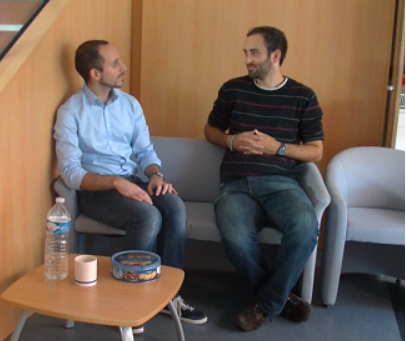
\includegraphics[width=0.7\linewidth]{./intention/actors.png} 
  \caption {Image représentant la configuration du scénario des cookies.}
  \label{fig:cookieScen}
\end{figure}

L'\textit{Événement de croyance divergente} a été montré aux utilisateurs et au robot entre le test \textit{Contextual clues} et le test \textit{Divergent belief Max}. 

Nous avons volontairement inclue une intention, \textit{Reading the book}, sans mettre de livre dans l'environnement visible, afin d'introduire un élément incertain dans le scénario.

\subsubsection{Scénario des clés}
\begin{itemize}

\item Objets: Une \textit{Boîte} est placée sur une \textit{Table}. La \textit{Boîte} cache partiellement la vue des personnes qui approchent. Un \textit{Livre} et un \textit{Mug} sont placés derrière la \textit{Boîte}, afin qu'ils puissent être vus depuis le \textit{Canapé} mais pas des gens qui s'approchent. Pour illustrer la configuration, une image extrait de la vidéo est présentée à la figure \ref{fig:keyScen}.

\item Intentions: prendre le \textit{Mug} \textit{Taking the mug}, prendre les \textit{clés} \textit{Taking the keys}, lire un \textit{Livre} \textit{Reading the book}.



\begin{figure}[ht!]
  \centering
 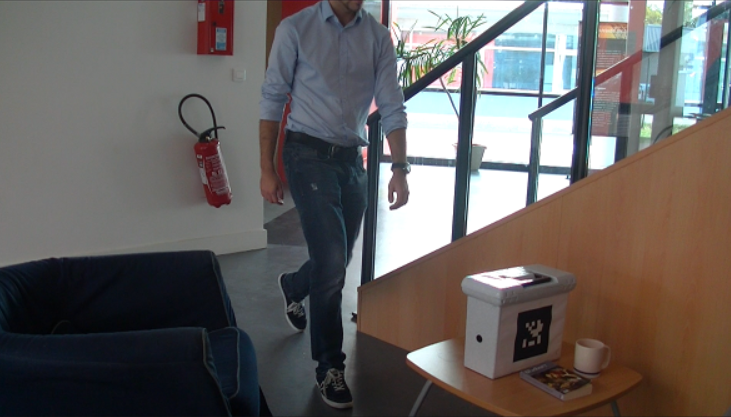
\includegraphics[width=0.8\linewidth]{./intention/keys1.png} 
  \caption {Image représentant la configuration du scénario des clés.}
  \label{fig:keyScen}
\end{figure}


\item Tests et événements:
\begin{itemize}
\item \textit{No clues}: \textit{Max} s'approche de la \textit{Table}.
\item\textit{Contextual clues}: \textit{Max} s'approche de la \textit{Table} en hâte, tout en enfilant un manteau.
\item \textit{Divergent belief Max}: \textit{Max} s'approche de la \textit{Table} en hâte, tout en enfilant un manteau.
\end{itemize}

\item \textit{Événements de croyance divergente}: \textit{Max} est assis sur le \textit{Canapé}, buvant dans le \textit{Mug}, et ayant les \textit{Clés} en mains. Son téléphone sonne, il pose les \textit{Clés} et le \textit{Mug} sur la \textit{Table}, derrière la \textit{Boîte}, et quitte la salle. Pendant que \textit{Max} est absent, \textit{Bob} arrive et prends place sur le \textit{Canapé}, lisant un \textit{Livre}. Lorsqu'il voit les \textit{Clés}, pose le \textit{Livre} sur la \textit{Table} et prends les \textit{Clés} pour les amener aux objets trouvés.
\end{itemize}

L'\textit{Événement de croyance divergente} est montré aux utilisateurs et au robot entre les événements de \textit{Contextual clues} et \textit{Divegent belief Max}.

\subsection{Étude utilisateurs}
Pour collecter les estimations d'intentions de la part d'humains, nous avons créer une étude en ligne, où nous présentons des vidéos en relation avec les tests et événements des deux scénarios. Les utilisateurs ont estimé la probabilité de chaque intention disponible sur une échelle de Likert à 5 niveaux. L'étude a été réalisée en trois langues, avec des utilisateurs résidents dans différents pays \footnote{Une version de cette étude est fournit à l'adresse http://goo.gl/forms/gWwdIutbOCUk3vdx2}. Nous avons recueilli les réponses de 78 adultes, calculé la moyenne de chaque réponse puis nous avons convertis ces moyennes en pourcentage, afin de les comparer aux réponses du robot.

Lorsqu'on observe les réponses des utilisateurs (voir figure \ref{fig:user_study_results}), nous observons que, dans l'absence d'indices, les individus ont donné la même note aux différentes intentions liées aux objets visibles. Les indices de contexte ont eu la plus grosse influence sur les réponses des utilisateurs. Cela est particulièrement visible dans le test \textit{Contextual Clues} du scénario des clés (\textit{Keys Scenario}), où les utilisateurs ont noté comme intention la plus probable \textit{Take Keys}, même si aucunes clés était visible dans la vidéo. Les croyances divergentes ont également influencé l'estimation des humains, mais dans une proportion moins importante. Globalement, les réponses les plus fortes, ont été données par le test \textit{Divergent Belief Max} sur le scénario des clés, qui utilise à la fois des indices de contexte et la connaissance de l'état mental divergent.

\subsection{Implémentation robotique}
\label{sec:expeRobotIntent}
Nous avons répliquer les deux scénarios avec un robot PR2 de Willow Garage\footnote{https://www.willowgarage.com/pages/pr2/overview}. Nous avons simplifier la perception, en utilisant de la capture de mouvement pour suivre les humains. Celle-ci est filtrée pour tenir compte des occlusions. Pour la détection d'objet nous utilisons un logiciel de reconnaissance de tags \footnote{Des vidéos d'expériences associées peuvent être vue sur  http://homepages.laas.fr/mfiore/roman2016.html}. 

Au début d'un scénario, le robot scanne l'environnement, construisant un modèle de l'état du monde. Avec notre perception, il n'est pas possible de savoir si la boîte de cookie est pleine ou vide et nous la considérons donc comme pleine au commencement d'un test, et ses valeurs sont mises à jour en utilisant les $postconditions$ des actions humaines inférées. Nous considérons que la boîte est vide lorsqu'un humain prends un cookie, et comme pleine lorsqu'un humain y a mis un cookie.

Nous avons construit différents IGs pour les scénarios. Chaque test a un graphe différent, lié à l'agent principal dont on veut reconnaître l'intention. Nous considérons trois différents nœuds de contexte pour ces IGs: \textit{HotDay}, qui est vrai lorsque la journée est particulièrement chaude; BreakTime, qui est vrai lorsque les agents prennent une pause; TimeToLeave, qui est vrai lorsqu'il est tard dans la journée, et que les humains partent en général de leur lieu de travail pour rentrer chez eux.

Comme indiqué précédemment, nous avons choisi de suivre \cite{Liu2014} afin d'apprendre le lien entre contexte et intention. Nous avons fait une petite étude utilisateur avec 15 personnes, dans laquelle 5 scénarios ont été présentés. Chaque scénario est lié à une des intentions utilisées dans nos tests. Pour chaque scénario, nous avons demander aux utilisateurs de noté le lien perçu entre l'intention et les trois contextes. Pour ce faire, les individus ont noté la "force" de ce lien sur une échelle de Likert à cinq niveaux. Nous avons utilisé la moyenne des réponses pour calculer la probabilité de la dépendance conditionnelle entre les nœuds de contexte et les nœuds d'intention.


Dans le scénario  du cookie (\textit{Cookie Scenario}) le graphe pour les tests est construit à partir des nœuds suivants:
\begin{itemize}
\item Nœuds de contexte: \textit{Hot Day}, \textit{Break Time}, \textit{Time to Leave}
\item Nœuds d'intention: \textit{Fill Cookie Box}, \textit{Eat Cookie}, \textit{Drink Water}, \textit{Read Book}.
\item Nœuds d'action: \textit{Move to Table}, \textit{Move to Kitchen}.
\item Nœuds d'observation: distance du corps de l'agent et de sa main à chaque cible d'action.
\end{itemize}

Nous introduisons l'intention de remplir la boîte de cookie (\textit{Fill Cookie Box}), qui n'est pas présente dans les tests soumis aux humains, afin que le robot détecte lorsque Bob remplit la boîte de cookies pendant l'événement de croyance divergente.

Notre robot, dans cette expérimentation, n'est pas équipé de capacité pour comprendre la parole de l'homme, et assigne directement les nœuds de contexte à des valeurs plausibles et qui pourrait être acquises en regardant les vidéos. Pour le test de \textit{Contextual Clues}, nous assignons la valeur de \textit{Hot Day} à vrai (dans la vidéo Max commente la chaleur du jour), et \textit{Break Time}, et \textit{Time to Leave} à faux (car aucun élément d'en la vidéo n'indique que ces contextes sont vrais).

%. Max and Bob seem to have taken a break from work before the other events are shown, in the Divergent Belief Event).

L'événement de croyance divergente (\textit{Divergent Belief Event}), le test \textit{Divergent Belief Max}, et le test \textit{Divergent Belief Bob} ont été montrés dans cet ordre au rorbot, qui a pu ainsi suivre et mettre à jour les états de croyances des agents et créer les nouveaux IGs qui conviennent à cette situation. Pendant l'événement de croyance divergente, plusieurs IGs ont étés créés avec différents nœuds d'action et d'observation, pour suivre la séquence d'action réalisée par les deux agents. Par exemple, quand \textit{Max} quitte la pièce, \textit{Bob} a la possibilité d'exécuter les actions \textit{Take Mug}, \textit{Take Water Bottle}, \textit{Open Cookie Box}, \textit{Move to Kitchen Shelf} ou \textit{Leave Room}. Les nœuds d'intention et de contexte restent quand à eux inchangés dans tous les IGs du scénario.


Le scénario des clés (\textit{Keys Scenario}) a un IG, avec les différences suivantes:
\begin{itemize}
\item Nœuds de contexte: \textit{Hot Day}, \textit{Break Time} et \textit{Time to Leave}.
\item Nœuds d'intention: \textit{Drink Water}, \textit{Take Keys}, \textit{Read Book}.
\end{itemize}

Les nœuds d'action et d'observation sont les même que le scénario précédent et suivent les mêmes idées durant l'événement de croyance divergente. Un exemple d'IG utilisé dans les tests est présenté à la figure \ref{fig:intention_graph}. Pour les tests \textit{Contextual Clues} et \textit{Divergent Belief}, nous mettons la valeur contextuelle \textit{Time to Leave} à vrai (Max mets un manteau et semble pressé), et les autres valeur contextuelle à faux. En utilisant le composant décrit dans les sections précédentes, et ces IGs, le robot a été capable d'obtenir des prédictions à partir des actions des utilisateurs.

\subsection{Discussion}
\label{discussion}
Nous réalisons des tests TOST pour chaque intention contenu dans les scénarios, en comparant les réponses des humains avec celles du robot pour un total de 21 tests.

Nous calculons les p-valeurs et réalisons nos tests en utilisant la valeur de signification $\alpha=0.05$.

En analysant les résultats de nos tests d'équivalence, présentés dans la figure \ref{fig:user_study_results}, des informations intéressantes peuvent en être extraites. 1) Le comportement de notre système est généralement proche des capacités humaines. 19 tests sur les 21 valident notre hypothèse avec une p-valeur inférieur à la valeur de signification. 2) Le contexte et l'état de croyance de l'homme sont à prendre en compte. Un système qui ignorerait ces deux facteurs aurait pu reconnaître correctement que l'intention du test \textit{No Clues}. 3) Certains raisonnement présent chez l'homme sont encore manquant dans notre système. Nous avons échoué à rejeter l'hypothèse nulle pour deux cas. Dans \textit{Divergent Belief Bob} les humains ont donné une note plus importante à l'intention \textit{Eat Cookie} que l'intention \textit{Drink Water}. Une explication est qu'ils ont penser que, étant donné que \textit{Bob} a rempli la \textit{Boîte de cookies}, il y a plus de chance qu'il souhaite manger un \textit{Cookie}. Cela permet de mettre en valeur que l'homme utilise des raisonnements temporels complexes pour évaluer l'intention, en considérant tout l'historique des actions des agents pour deviner leur intention.



 \begin{figure}[h!]
	\centering
	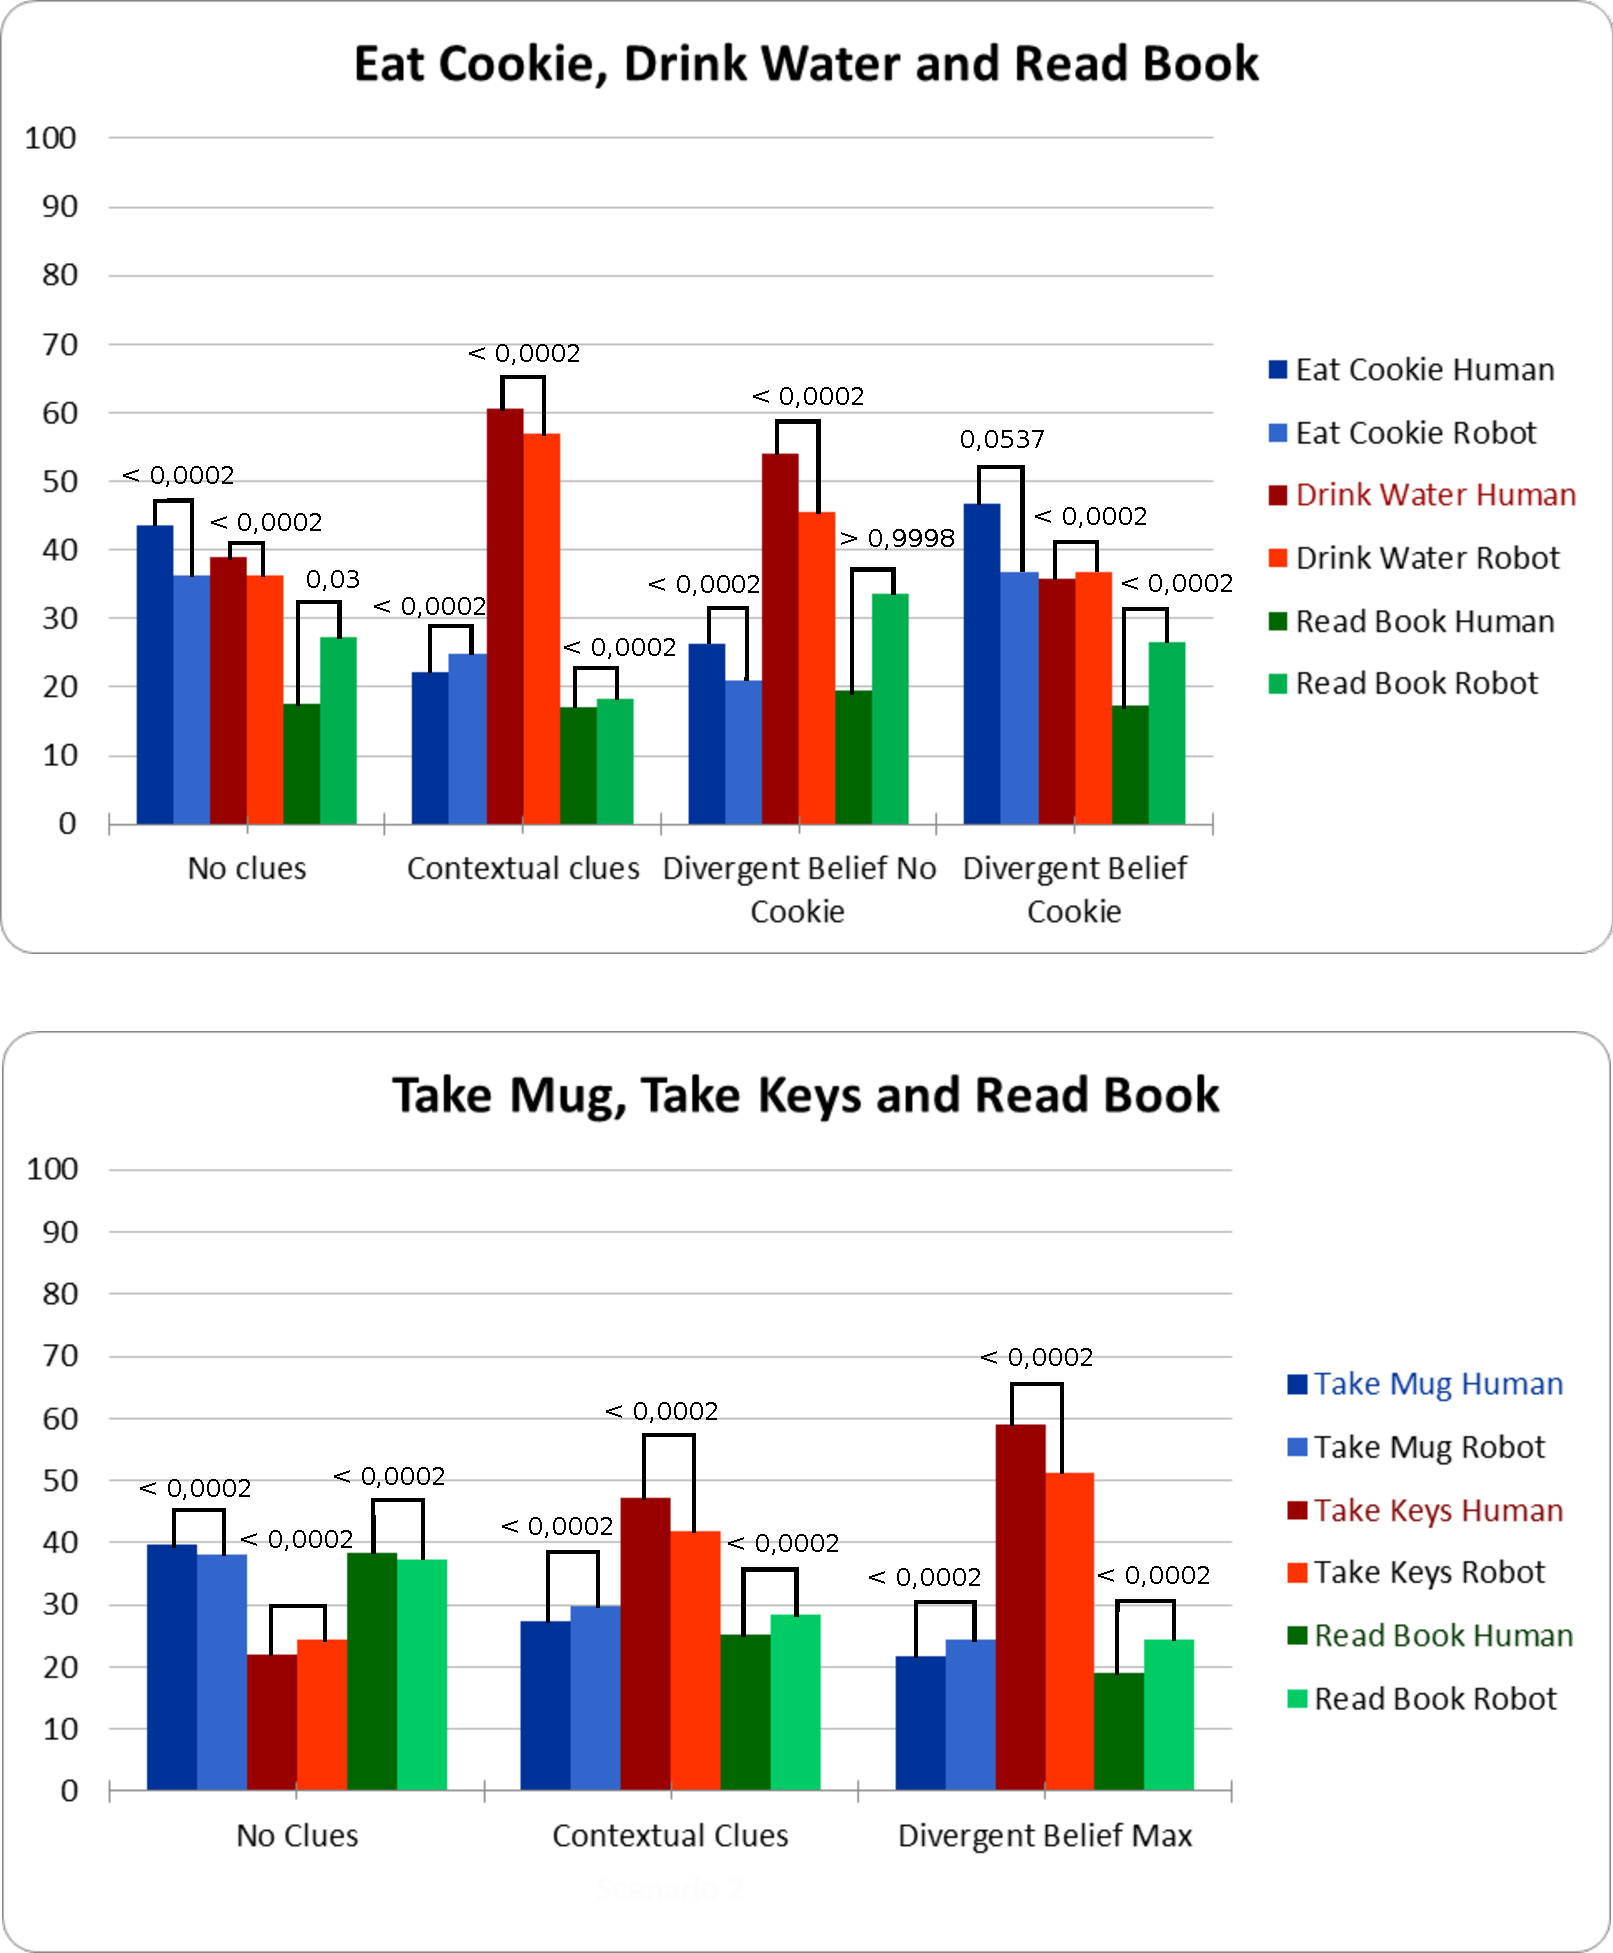
\includegraphics[clip,scale=0.52]{img/pvalues1.pdf}
	\caption{Résultats expérimentaux. Les résultats pour les deux scénarios sont représentés sous forme de graphes. Les intentions, estimés par les hommes et le robot, sont représentées sous différentes couleurs (voir légende). L'estimation des mêmes intentions par le robot et par les hommes sont placées côtes à côtes. Chaque colonne représente la probabilité d'une intention exprimé en pour-cent. Les P-valeurs du test d'équivalence sont ajoutées au graphe.}
	\label{fig:user_study_results}
  	\vspace{-16pt}
\end{figure}


\section{Conclusion}
Dans ce chapitre, nous avons présenté un système capable d'évaluer les intentions humaines en utilisant la gestion de la croyance, les données contextuelles et l'observation d'actions. Nous avons effectué une étude sur les utilisateurs où nous avons comparé les prédictions de notre système avec ceux des humains. Dans cette étude, nous avons montré que notre système est en mesure, dans plusieurs situations, d'approcher les capacités humaines. Notre système utilise la prédiction de l'intention afin d'aider de manière proactive les humains à atteindre leurs objectifs en effectuant une partie du plan ou en corrigeant verbalement leur état de croyance.

Les résultats obtenus mettent également en valeur que les humains utilisent probablement des raisonnements temporels pour désambiguïser les intentions (comme indiqué dans la section \ref{discussion}). Il serait intéressant d'étudier d'avantage ces mécanismes et d'utiliser notre base de données temporelles présentée en \ref{sec:dbt} pour ajouter ce type de mécanisme au robot.

Nous supposons, dans ce travail, que le robot a toujours un état de croyance correcte et l'utilise comme une référence pour l'état de l'environnement. Il serait intéressant d'aborder le problème où le robot a un état de croyance erronée, par exemple en analysant le degré de confiance que l'homme semble avoir dans ses comportements.


% In this paper we presented a system able to assess human intentions using belief management, contextual data and action observation. We performed a user study where we compared the predictions of our system with those of humans. In this study, we showed that our system is able, in several situations, to approach human capacities. Our system uses intention prediction to proactively help humans achieve their goals by performing a part of the plan or verbally correcting their belief state.

% The system is flexible and easily extendable by adding new MDP models and planning domains intentions. Most of the computation regarding MDPs is done offline, by calculating the action value functions and storing them in tables, with online computation mainly used for situation assessment, which uses efficient algorithms. Thanks to these aspects our system would be able to include more intentions and to maintain real-time performances.

% There are several possible developments to our system. We could explore the use of more complex models, for example by considering mental beliefs as probabilistic, while trying to maintain an efficient computation time. Learning algorithm could also contribute to our system, by allowing the robot to adapt its recognition process to the behaviors of different users. The result also puts into light that humans might use deeper temporal reasoning to disambiguate intentions (as discussed in section \ref{discussion}), which should be further studied.

% We assume, in this work, that the robot has always a correct belief state and uses it as a reference for the state of the environment. It would be interesting to address the problem where the robot has a wrong belief state, for example by analyzing the degree of confidence that the human seems to have in his behaviors.

\ifdefined\included
\else
\bibliographystyle{acm}
\bibliography{These}
\end{document}
\fi
